\documentclass[a4paper,twoside,twocolumn]{article}

\usepackage{times}
\usepackage{color}
\usepackage{graphicx}
\usepackage{alltt}
\usepackage{textcomp}
\usepackage{drawstack}
\usepackage{float}

\usepackage{a4med}
\usepackage{comp-tut}

\renewcommand{\textfraction}{0.0}
\renewcommand{\floatpagefraction}{1.0}
\renewcommand{\dblfloatpagefraction}{1.0}
\renewcommand{\topfraction}{1.0}
\renewcommand{\dbltopfraction}{1.0}
\setcounter{topnumber}{3}
\setcounter{dbltopnumber}{3}
\setcounter{totalnumber}{3}

\newcommand{\figurerule}{\rule{\textwidth}{0.5pt}}
\newcommand{\OPN}[1]{\textbf{#1}}
%\newcommand{\OP}[2]{\item[#1]}
\newcommand{\OP}[2]{\item[#1]}% (#2)}

\newcommand{\nb}[1]{}
%\renewcommand{\nb}[1]{{\color{blue}#1}}
\newcommand{\LT}{$<$}

\begin{document}

\thispagestyle{empty}
\title{\vspace*{-3cm}Interpreter}
\author{Brae Webb}
\maketitle
\pagestyle{myheadings}
\vspace*{-4ex}

An interpreter is a type of program, similar to a compiler, which builds an
abstract syntax tree from input source code. An interpreter differs from a
compiler in that it does not generate machine code. Instead it will evaluate
the expression nodes and execute the statement nodes in an abstract syntax tree
directly in order to run a program.


The PL0 Abstract Syntax Tree (AST) is comprised of expression nodes
(\texttt{ExpNode}) and statement nodes (\texttt{StatementNode}). The PL0
Interpreter uses a visitor pattern to visit each of the statement and expression
nodes.

\section{Evaluating Expression Nodes}\label{section:expressions}
When an expression node is visited it is evaluated into an \texttt{Integer}.
Expression nodes consist of atomic and composite nodes. Atomic nodes retrieve
their values from variable lookup or user input, examples are the 
\texttt{VariableNode} and \texttt{ReadNode}. Composite nodes are derived from
other composite nodes or atomic nodes, examples are the \texttt{OperatorNode}
and \texttt{DereferenceNode}.

%An expression node is visited by calling the 
%\emph{.evaluate(ExpTransform$\langle$Integer$\rangle$)} method of the node.

\begin{figure}[H]
\begin{java}
public Integer visitReadNode(ExpNode
        .ReadNode node) {
    beginExec("Read");
    /* Read next int from input stream */
    int result;
    try {
        result = Integer
                .parseInt(in.readLine());
    } catch (Exception e) {
        runtime("read value not int",
                node.getLocation(),
                currentFrame);
        return -1; // Never reached
    }
    endExec("Read");
    return result;
}
\end{java}
\caption{Evaluating a \texttt{ReadNode}}\label{figure:readnode}
\end{figure}

\section{Executing Statement Nodes}\label{section:statements}
When a statement node is visited it executes Java code that simulates the
behaviour of the node it represents in PL0. For example, a \texttt{WriteNode}
will evaluate its \texttt{ExpNode} and print the result to the output.

\begin{figure}[H]
\begin{java}
public void visitWriteNode(StatementNode
        .WriteNode node) {
    beginExec("Write");
    /* Evaluate the code in the
     * write expression */
    int result = node.getExp()
            .evaluate(this);
    /* Print the result to the 
     * output stream */
    outStream.println(result);
    endExec("Write");
}
\end{java}
\caption{Executing a \texttt{WriteNode}}\label{figure:writenode}
\end{figure}

\section{Interpreter Frame}\label{section:frame}

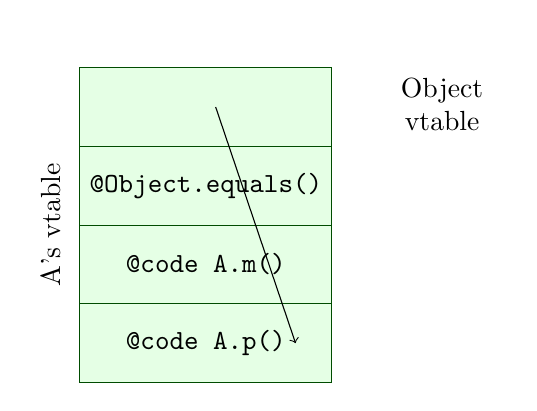
\begin{tikzpicture}
  \draw (3, -1) node (Otm) {
    \begin{tabular}{c}
      Object\\vtable
    \end{tabular}
  };

  \drawstruct{(0,0)}
  \structcell[freecell]{~} \coordinate (Atm) at (currentcell.east);
  \structcell[freecell]{\texttt{@Object.equals()}}
  \structcell[freecell]{\texttt{@code A.m()}}
  \structcell[freecell]{\texttt{@code A.p()}} \coordinate (A) at (currentcell.east);
  \structname{
    \begin{tabular}{c}
      A's vtable
    \end{tabular}
  }

  \draw[->] (Atm) -- (A);
\end{tikzpicture}

\end{document}